\documentclass[]{article}
\usepackage{lmodern}
\usepackage{amssymb,amsmath}
\usepackage{ifxetex,ifluatex}
\usepackage{fixltx2e} % provides \textsubscript
\ifnum 0\ifxetex 1\fi\ifluatex 1\fi=0 % if pdftex
  \usepackage[T1]{fontenc}
  \usepackage[utf8]{inputenc}
\else % if luatex or xelatex
  \ifxetex
    \usepackage{mathspec}
  \else
    \usepackage{fontspec}
  \fi
  \defaultfontfeatures{Ligatures=TeX,Scale=MatchLowercase}
\fi
% use upquote if available, for straight quotes in verbatim environments
\IfFileExists{upquote.sty}{\usepackage{upquote}}{}
% use microtype if available
\IfFileExists{microtype.sty}{%
\usepackage{microtype}
\UseMicrotypeSet[protrusion]{basicmath} % disable protrusion for tt fonts
}{}
\usepackage[margin=1in]{geometry}
\usepackage{hyperref}
\hypersetup{unicode=true,
            pdftitle={Microplastics in Lettuce},
            pdfauthor={Susannah Budd},
            pdfborder={0 0 0},
            breaklinks=true}
\urlstyle{same}  % don't use monospace font for urls
\usepackage{graphicx,grffile}
\makeatletter
\def\maxwidth{\ifdim\Gin@nat@width>\linewidth\linewidth\else\Gin@nat@width\fi}
\def\maxheight{\ifdim\Gin@nat@height>\textheight\textheight\else\Gin@nat@height\fi}
\makeatother
% Scale images if necessary, so that they will not overflow the page
% margins by default, and it is still possible to overwrite the defaults
% using explicit options in \includegraphics[width, height, ...]{}
\setkeys{Gin}{width=\maxwidth,height=\maxheight,keepaspectratio}
\IfFileExists{parskip.sty}{%
\usepackage{parskip}
}{% else
\setlength{\parindent}{0pt}
\setlength{\parskip}{6pt plus 2pt minus 1pt}
}
\setlength{\emergencystretch}{3em}  % prevent overfull lines
\providecommand{\tightlist}{%
  \setlength{\itemsep}{0pt}\setlength{\parskip}{0pt}}
\setcounter{secnumdepth}{0}
% Redefines (sub)paragraphs to behave more like sections
\ifx\paragraph\undefined\else
\let\oldparagraph\paragraph
\renewcommand{\paragraph}[1]{\oldparagraph{#1}\mbox{}}
\fi
\ifx\subparagraph\undefined\else
\let\oldsubparagraph\subparagraph
\renewcommand{\subparagraph}[1]{\oldsubparagraph{#1}\mbox{}}
\fi

%%% Use protect on footnotes to avoid problems with footnotes in titles
\let\rmarkdownfootnote\footnote%
\def\footnote{\protect\rmarkdownfootnote}

%%% Change title format to be more compact
\usepackage{titling}

% Create subtitle command for use in maketitle
\providecommand{\subtitle}[1]{
  \posttitle{
    \begin{center}\large#1\end{center}
    }
}

\setlength{\droptitle}{-2em}

  \title{Microplastics in Lettuce}
    \pretitle{\vspace{\droptitle}\centering\huge}
  \posttitle{\par}
    \author{Susannah Budd}
    \preauthor{\centering\large\emph}
  \postauthor{\par}
      \predate{\centering\large\emph}
  \postdate{\par}
    \date{05/04/2019}


\begin{document}
\maketitle

\hypertarget{abstract}{%
\paragraph{Abstract}\label{abstract}}

\hypertarget{introduction}{%
\paragraph{Introduction}\label{introduction}}

\hypertarget{methods}{%
\paragraph{Methods}\label{methods}}

\begin{enumerate}
\def\labelenumi{\arabic{enumi}.}
\tightlist
\item
  Obtain Romaine lettuce. Purchase two unpackaged heads of romaine
  lettuce and two heads of romaine lettuce in plastic packaging
  (pre-chopped for salad is acceptable) from 5 nearby stores - Sprouts
  on Foothill Boulevard, Stater Bros.~on N. Garey Avenue, Cardenas on E.
  Holt Avenue, El Super on E. Holt Avenue, and Super King on Auto Center
  Drive. Upon purchasing the lettuce, ensure that it is carried out in
  individual paper bags to avoid contamination. Seal the bags to avoid
  contamination with airborne particulates, however, some contamination
  will likely be unavoidable.~
\item
  In the lab, obtain a glass blender. If unbagged, thoroughly wash one
  head of lettuce with deionized water, and then fill the blender with
  leaves until they reach the top. If bagged insert leaves into blender
  until they reach the top without washing, as the lettuce is labeled
  pre-washed.~
\item
  Add 200 mL of Milli-Q deionized water to the blender. Blend for 30
  seconds on the slower ``grind'' setting, then for 60 seconds on the
  faster ``cream'' setting.~
\item
  Strain the contents of each beaker through a stainless steel filter
  with a mesh size of 5 mm to capture larger organic fibers while
  allowing all particles meeting the qualification of ``microplastic''
  (\textgreater{}5mm) to pass through until 100 mL of solution is
  obtained. Place this solution in a glass beaker covered with aluminum
  foil to avoid airborne contamination.~
\item
  Extract 5 mL of the blended lettuce solution using a glass pipette and
  place in a 100 mL glass beaker. Due to the large quantities of
  cellulose in lettuce, use the enzyme cellulase from Niger Aspergillus
  niger to digest the remaining organic material while leaving any
  microplastic particles intact. Add 5 mL of cellulase and 10 mL of a
  phosphate-buffered saline (PBS) solution (1 L prepared with 8 g sodium
  chloride, 200 mg potassium chloride, 1.44 g disodium phosphate and 240
  mg monopotassium phosphate in deionized water, set to pH 5.0 using
  hydrochloric acid). Cover beaker with aluminum foil.~
\item
  Incubate the solution at 50° C for 4 days.~
\item
  Repeat steps 2-6 for every purchased head of lettuce.~
\item
  Add NaCl in solution with deionized water (density=1.2g/mL, stirred
  for 10 minutes) to the incubated solution until the beaker has 100 mL
  of solution in it. Allow solution to settle for 30 minutes, then use a
  vacuum system to collect the top 40 mL of each sample and any floating
  microplastics within it.~9. Add 5 mL of 0.08 g/mL Nile red dye
  solution to this extracted solution and wait 30 minutes to allow
  staining to occur.~
\item
  Run this extracted and stained solution through vacuum filtration with
  an entirely glass apparatus to separate stained fibers from their
  liquid matrix. Place the resulting filter paper in a glass beaker,
  cover with aluminium foil, and allow it to dry overnight.~
\item
  Use RStudio to generate random coordinate points. Create a grid on the
  dried filter paper, and plot four random points onto this grid on each
  paper.~
\item
  Use the digital Revolve microscope with fluorescent light (4x zoom
  lens, TXRED fluorescent/FL overlay at 100\% brightness, 110 ms
  capture) and use ocular techniques to count the number of fluorescent
  particles present at each marked location on the paper.~
\item
  Repeat steps 8-12 with each incubated solution.~
\item
  In order to mitigate the impacts of contamination or procedural error,
  corroborated the results through the use of blanks. 3 water
  ``samples'' should go through steps 2-11 alongside the experimental
  samples, but with 100 mL of deionized water rather than solution
  material. All equipment used should be washed thoroughly before and
  after touching any sample, and all water used to wash should be
  deionized so as to avoid contamination from the water.~
\item
  The methods of Löder et al.~2017, Maes et al.~2017, Wang and Wang
  2018, Karlsson et al.~2017, and Quinn et al.~2018 were consulted in
  developing these proposed procedures.
\end{enumerate}

\hypertarget{results}{%
\paragraph{Results}\label{results}}

The data collection yielded five replicates and five pseudo-replicates
for both bagged and unbagged lettuce, as two bagged and unbagged heads
were purchased at five different stores. In order to more accurately
reflect these replicates, the number of microplastics found on each head
of lettuce was averaged with its pair. For example, the number of
microplastics found on each bagged lettuce head purchased at Cardenas
were averaged with one another. The graph below shows the box plots of
these averages for bagged and unbagged lettuce.

\begin{center}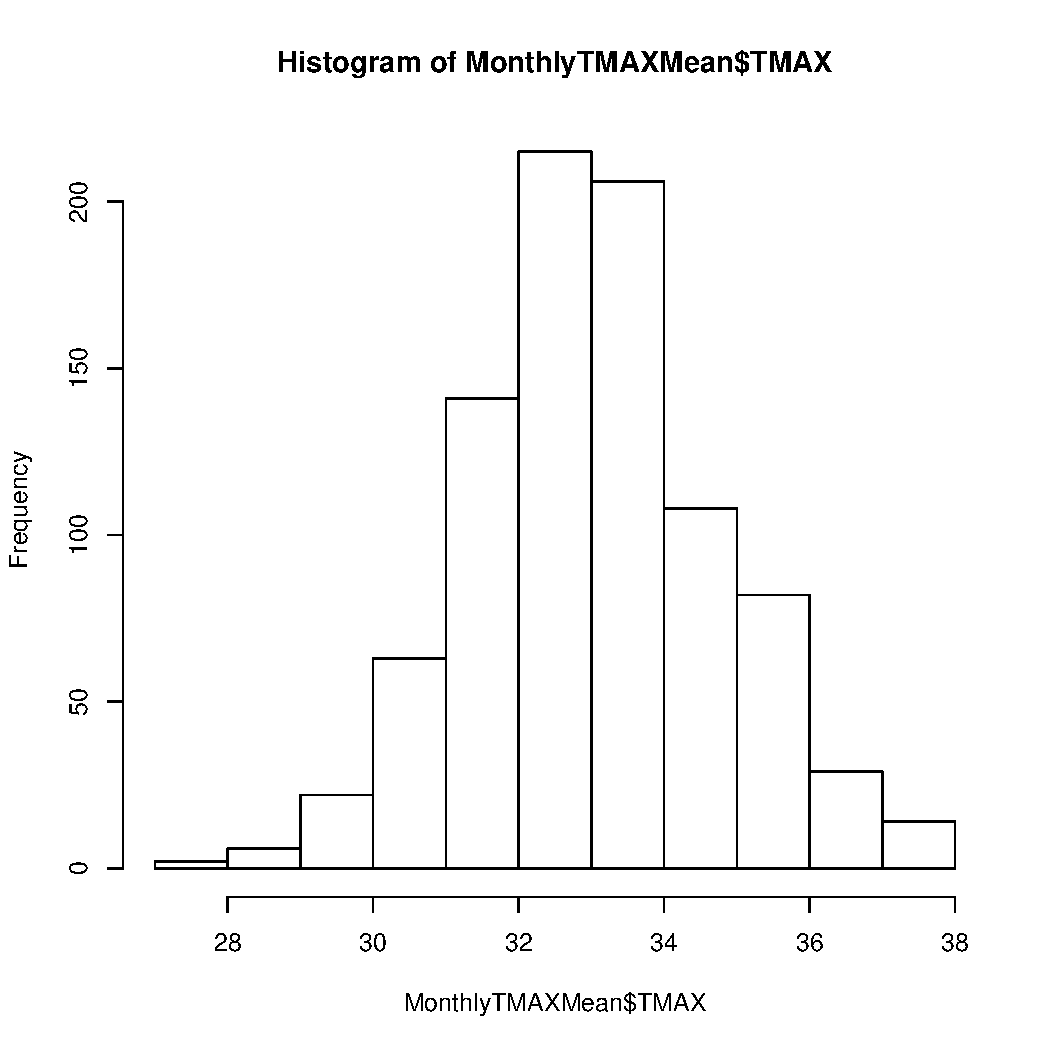
\includegraphics{Lab_Report_files/figure-latex/unnamed-chunk-2-1} \end{center}

\hypertarget{normality-tests}{%
\paragraph{\texorpdfstring{Normality Tests\\
}{Normality Tests }}\label{normality-tests}}

This experiment was designed to test the null hypothesis of ``there is
no difference in microplastic quantities in romaine lettuce with or
without plastic packaging.'' In order to determine whether or not to
reject the null hypothesis, whether or not the data fell within normal
distribution was first assessed, using Q-Q Plots and the Shapiro-Wilk
normality test.

\hypertarget{bagged}{%
\subparagraph{Bagged}\label{bagged}}

For bagged lettuce data, the Shapiro-Wilk normality test yielded a
p-value of 0.2768, indicating that it is within the bounds of normal
distribution. The Q-Q plot, shown below, also demonstrates that most
points fall within the expected bounds.

\begin{center}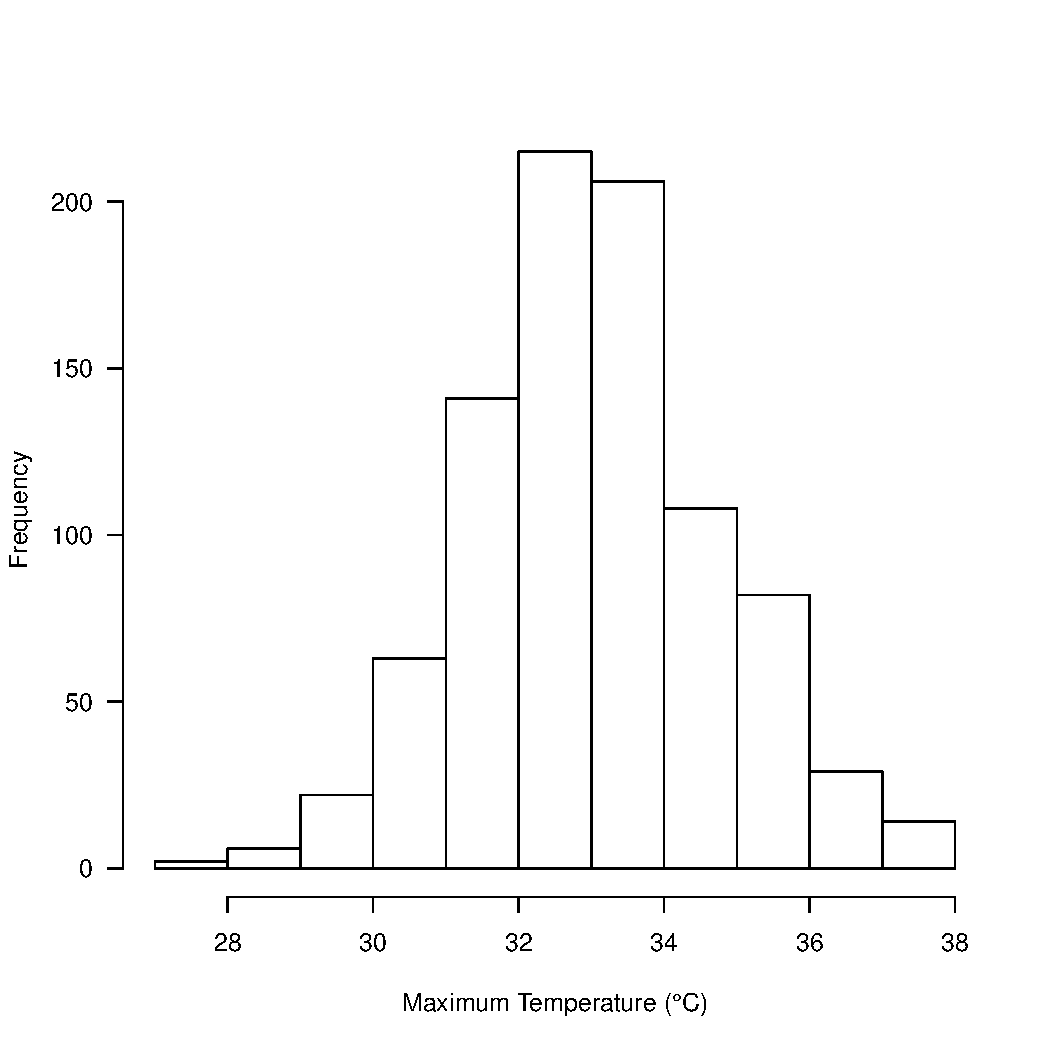
\includegraphics{Lab_Report_files/figure-latex/unnamed-chunk-3-1} \end{center}

\hypertarget{unbagged}{%
\subparagraph{Unbagged}\label{unbagged}}

For unbagged lettuce data, the Shapiro-Wilk normality test yielded a
p-value of 0.04526, indicating that it is not within the bounds of
normal distribution. The Q-Q plot, shown below, also demonstrates that,
while most points fall within the expected bounds, some are much further
out of normal distribution than they were for the bagged lettuce data.

\begin{center}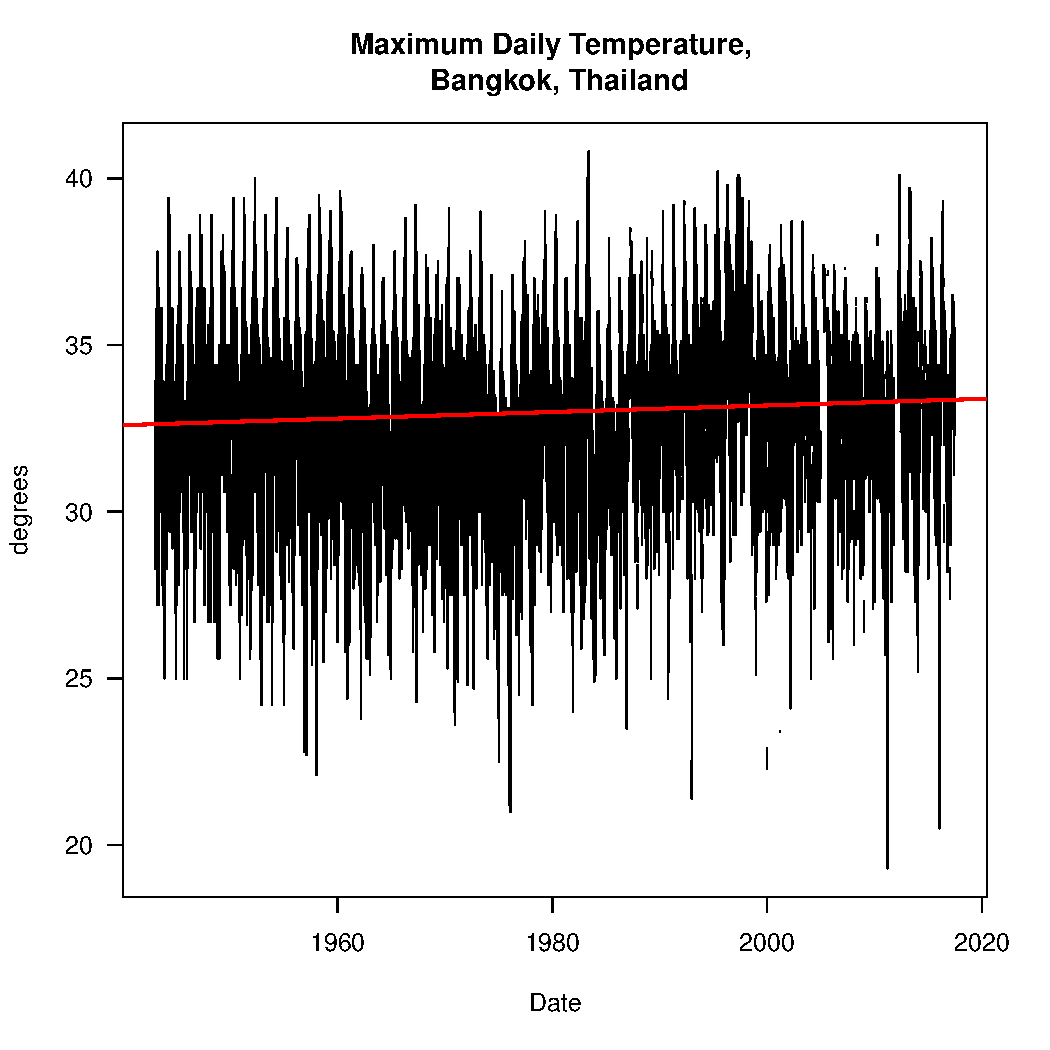
\includegraphics{Lab_Report_files/figure-latex/unnamed-chunk-5-1} \end{center}

\hypertarget{statistical-analysis}{%
\paragraph{Statistical Analysis}\label{statistical-analysis}}

As the unbagged data fell outside of normal distribution, a Paired
Samples Wilcoxon Test was used to evaluate the data. Using this test, a
p-value of 0.5839 was yielded. This p-value does not demonstrate
statistical significance, meaning that the null hypothesis may not be
rejected. A Two-Sample T-Test was also conducted, yielding a p-value of
0.2538. This also does not demonstrate statistical significance,
indicating that statistical significance likely would not be
demonstrated even if the data fell within normal distribution.

\hypertarget{discussion}{%
\paragraph{Discussion}\label{discussion}}

\hypertarget{conclusion}{%
\paragraph{Conclusion}\label{conclusion}}


\end{document}
